% SOURCE: quant_survival_repair_v1.json fields cells[*].arms[*].absolute_quantized_esr.point; cells[*].arms[*].conditional_survival_given_fp32_worked.point.
% SOURCE: quant_survival_repair_v1.json fields module_provenance.version; module_provenance.n_boot (asserted v1.2.1 and 500).
% !TEX encoding = UTF-8 Unicode
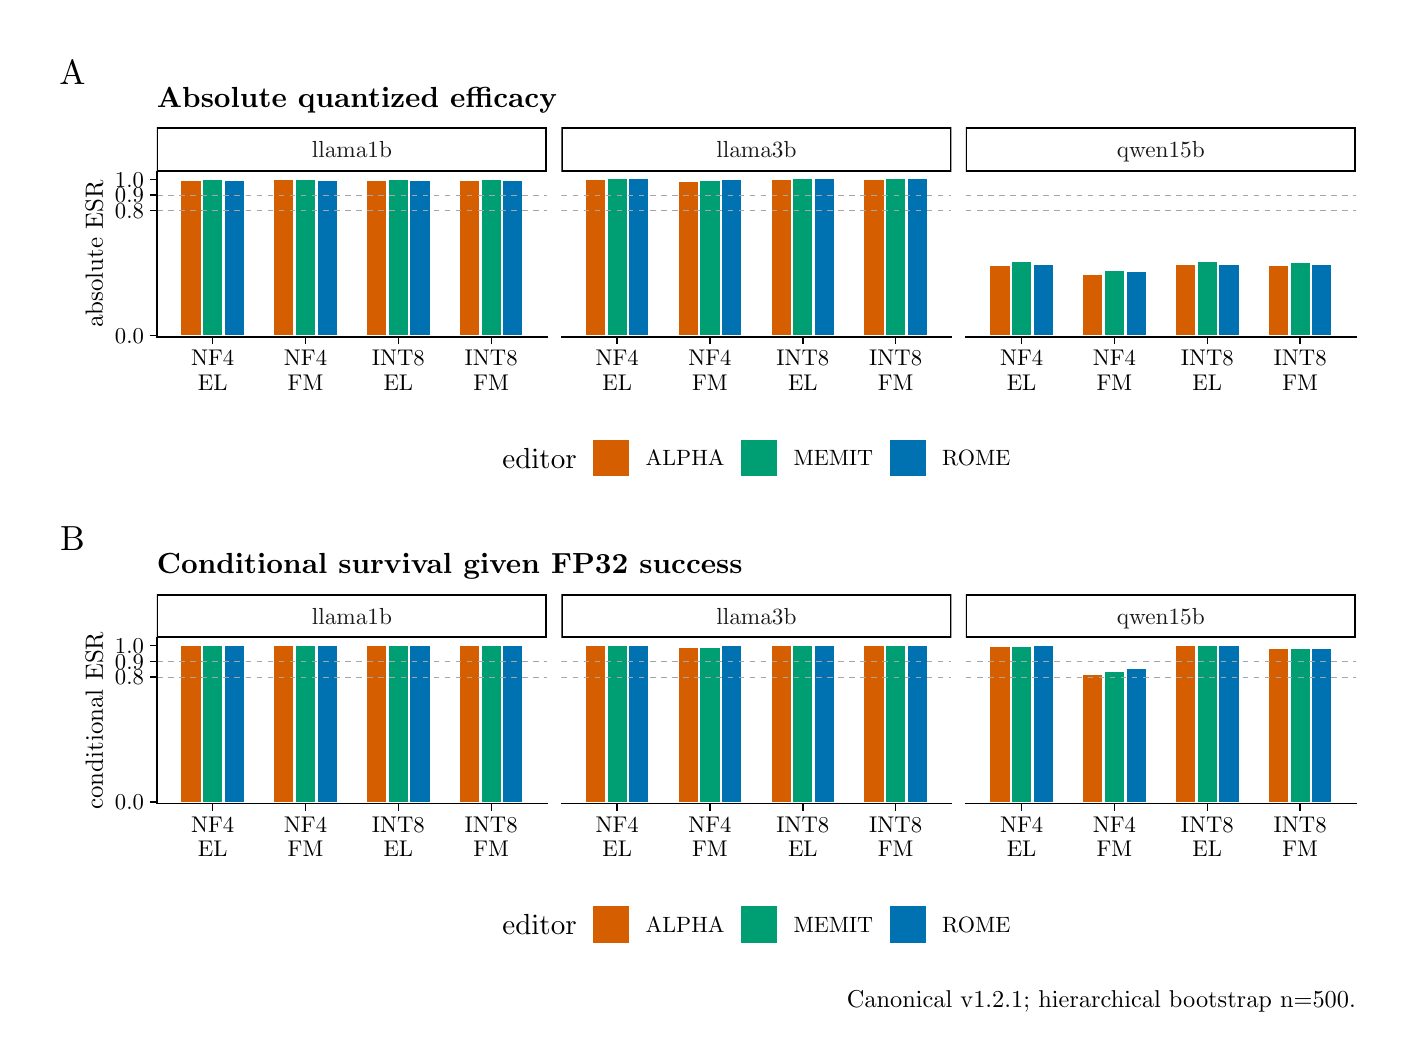
\begin{tikzpicture}[x=1pt,y=1pt]
\definecolor{fillColor}{RGB}{255,255,255}
\path[use as bounding box,fill=fillColor,fill opacity=0.00] (0,0) rectangle (491.44,361.35);
\begin{scope}
\path[clip] (  0.00,  0.00) rectangle (491.44,361.35);
\definecolor{drawColor}{RGB}{255,255,255}
\definecolor{fillColor}{RGB}{255,255,255}

\path[draw=drawColor,line width= 0.6pt,line join=round,line cap=round,fill=fillColor] (  0.00, -0.00) rectangle (491.44,361.35);
\end{scope}
\begin{scope}
\path[clip] (  5.50,187.31) rectangle (485.94,355.85);
\definecolor{drawColor}{RGB}{255,255,255}
\definecolor{fillColor}{RGB}{255,255,255}

\path[draw=drawColor,line width= 0.5pt,line join=round,line cap=round,fill=fillColor] (  5.50,187.31) rectangle (485.94,355.85);
\end{scope}
\begin{scope}
\path[clip] (  5.50, 18.77) rectangle (485.94,187.31);
\definecolor{drawColor}{RGB}{255,255,255}
\definecolor{fillColor}{RGB}{255,255,255}

\path[draw=drawColor,line width= 0.5pt,line join=round,line cap=round,fill=fillColor] (  5.50, 18.77) rectangle (485.94,187.31);
\end{scope}
\begin{scope}
\path[clip] ( 46.72,249.59) rectangle (187.63,309.37);
\definecolor{fillColor}{RGB}{255,255,255}

\path[fill=fillColor] ( 46.72,249.59) rectangle (187.63,309.37);
\definecolor{fillColor}{RGB}{213,94,0}

\path[fill=fillColor] ( 55.56,250.15) rectangle ( 62.49,306.08);

\path[fill=fillColor] ( 89.10,250.15) rectangle ( 96.04,306.17);

\path[fill=fillColor] (122.65,250.15) rectangle (129.59,306.08);

\path[fill=fillColor] (156.20,250.15) rectangle (163.14,306.08);
\definecolor{fillColor}{RGB}{0,158,115}

\path[fill=fillColor] ( 63.38,250.15) rectangle ( 70.32,306.27);

\path[fill=fillColor] ( 96.93,250.15) rectangle (103.87,306.17);

\path[fill=fillColor] (130.48,250.15) rectangle (137.41,306.27);

\path[fill=fillColor] (164.03,250.15) rectangle (170.96,306.27);
\definecolor{fillColor}{RGB}{0,114,178}

\path[fill=fillColor] ( 71.21,250.15) rectangle ( 78.15,306.08);

\path[fill=fillColor] (104.76,250.15) rectangle (111.69,306.08);

\path[fill=fillColor] (138.31,250.15) rectangle (145.24,306.08);

\path[fill=fillColor] (171.86,250.15) rectangle (178.79,306.08);
\definecolor{drawColor}{gray}{0.65}

\path[draw=drawColor,line width= 0.3pt,dash pattern=on 2pt off 2pt ,line join=round] ( 46.72,295.27) -- (187.63,295.27);

\path[draw=drawColor,line width= 0.3pt,dash pattern=on 2pt off 2pt ,line join=round] ( 46.72,300.91) -- (187.63,300.91);
\end{scope}
\begin{scope}
\path[clip] (192.88,249.59) rectangle (333.78,309.37);
\definecolor{fillColor}{RGB}{255,255,255}

\path[fill=fillColor] (192.88,249.59) rectangle (333.78,309.37);
\definecolor{fillColor}{RGB}{213,94,0}

\path[fill=fillColor] (201.71,250.15) rectangle (208.64,306.36);

\path[fill=fillColor] (235.26,250.15) rectangle (242.19,305.70);

\path[fill=fillColor] (268.81,250.15) rectangle (275.74,306.36);

\path[fill=fillColor] (302.36,250.15) rectangle (309.29,306.36);
\definecolor{fillColor}{RGB}{0,158,115}

\path[fill=fillColor] (209.54,250.15) rectangle (216.47,306.55);

\path[fill=fillColor] (243.09,250.15) rectangle (250.02,305.80);

\path[fill=fillColor] (276.64,250.15) rectangle (283.57,306.55);

\path[fill=fillColor] (310.18,250.15) rectangle (317.12,306.55);
\definecolor{fillColor}{RGB}{0,114,178}

\path[fill=fillColor] (217.37,250.15) rectangle (224.30,306.55);

\path[fill=fillColor] (250.92,250.15) rectangle (257.85,306.36);

\path[fill=fillColor] (284.46,250.15) rectangle (291.40,306.55);

\path[fill=fillColor] (318.01,250.15) rectangle (324.95,306.55);
\definecolor{drawColor}{gray}{0.65}

\path[draw=drawColor,line width= 0.3pt,dash pattern=on 2pt off 2pt ,line join=round] (192.88,295.27) -- (333.78,295.27);

\path[draw=drawColor,line width= 0.3pt,dash pattern=on 2pt off 2pt ,line join=round] (192.88,300.91) -- (333.78,300.91);
\end{scope}
\begin{scope}
\path[clip] (339.03,249.59) rectangle (479.94,309.37);
\definecolor{fillColor}{RGB}{255,255,255}

\path[fill=fillColor] (339.03,249.59) rectangle (479.94,309.37);
\definecolor{fillColor}{RGB}{213,94,0}

\path[fill=fillColor] (347.87,250.15) rectangle (354.80,275.34);

\path[fill=fillColor] (381.41,250.15) rectangle (388.35,271.86);

\path[fill=fillColor] (414.96,250.15) rectangle (421.90,275.62);

\path[fill=fillColor] (448.51,250.15) rectangle (455.45,275.34);
\definecolor{fillColor}{RGB}{0,158,115}

\path[fill=fillColor] (355.69,250.15) rectangle (362.63,276.56);

\path[fill=fillColor] (389.24,250.15) rectangle (396.18,273.27);

\path[fill=fillColor] (422.79,250.15) rectangle (429.72,276.56);

\path[fill=fillColor] (456.34,250.15) rectangle (463.27,276.38);
\definecolor{fillColor}{RGB}{0,114,178}

\path[fill=fillColor] (363.52,250.15) rectangle (370.46,275.53);

\path[fill=fillColor] (397.07,250.15) rectangle (404.00,272.99);

\path[fill=fillColor] (430.62,250.15) rectangle (437.55,275.62);

\path[fill=fillColor] (464.17,250.15) rectangle (471.10,275.53);
\definecolor{drawColor}{gray}{0.65}

\path[draw=drawColor,line width= 0.3pt,dash pattern=on 2pt off 2pt ,line join=round] (339.03,295.27) -- (479.94,295.27);

\path[draw=drawColor,line width= 0.3pt,dash pattern=on 2pt off 2pt ,line join=round] (339.03,300.91) -- (479.94,300.91);
\end{scope}
\begin{scope}
\path[clip] ( 46.72,309.37) rectangle (187.63,325.19);
\definecolor{drawColor}{RGB}{0,0,0}
\definecolor{fillColor}{RGB}{255,255,255}

\path[draw=drawColor,line width= 1.1pt,line join=round,line cap=round,fill=fillColor] ( 46.72,309.37) rectangle (187.63,325.19);
\definecolor{drawColor}{gray}{0.10}

\node[text=drawColor,anchor=base,inner sep=0pt, outer sep=0pt, scale=  0.84] at (117.17,314.38) {llama1b};
\end{scope}
\begin{scope}
\path[clip] (192.88,309.37) rectangle (333.78,325.19);
\definecolor{drawColor}{RGB}{0,0,0}
\definecolor{fillColor}{RGB}{255,255,255}

\path[draw=drawColor,line width= 1.1pt,line join=round,line cap=round,fill=fillColor] (192.88,309.37) rectangle (333.78,325.19);
\definecolor{drawColor}{gray}{0.10}

\node[text=drawColor,anchor=base,inner sep=0pt, outer sep=0pt, scale=  0.84] at (263.33,314.38) {llama3b};
\end{scope}
\begin{scope}
\path[clip] (339.03,309.37) rectangle (479.94,325.19);
\definecolor{drawColor}{RGB}{0,0,0}
\definecolor{fillColor}{RGB}{255,255,255}

\path[draw=drawColor,line width= 1.1pt,line join=round,line cap=round,fill=fillColor] (339.03,309.37) rectangle (479.94,325.19);
\definecolor{drawColor}{gray}{0.10}

\node[text=drawColor,anchor=base,inner sep=0pt, outer sep=0pt, scale=  0.84] at (409.48,314.38) {qwen15b};
\end{scope}
\begin{scope}
\path[clip] (  0.00,  0.00) rectangle (491.44,361.35);
\definecolor{drawColor}{RGB}{0,0,0}

\path[draw=drawColor,line width= 0.5pt,line join=round,line cap=rect] ( 46.72,249.59) --
	(187.63,249.59);
\end{scope}
\begin{scope}
\path[clip] (  0.00,  0.00) rectangle (491.44,361.35);
\definecolor{drawColor}{RGB}{0,0,0}

\path[draw=drawColor,line width= 0.5pt,line join=round] ( 66.85,246.96) --
	( 66.85,249.59);

\path[draw=drawColor,line width= 0.5pt,line join=round] (100.40,246.96) --
	(100.40,249.59);

\path[draw=drawColor,line width= 0.5pt,line join=round] (133.95,246.96) --
	(133.95,249.59);

\path[draw=drawColor,line width= 0.5pt,line join=round] (167.50,246.96) --
	(167.50,249.59);
\end{scope}
\begin{scope}
\path[clip] (  0.00,  0.00) rectangle (491.44,361.35);
\definecolor{drawColor}{RGB}{0,0,0}

\node[text=drawColor,anchor=base,inner sep=0pt, outer sep=0pt, scale=  0.82] at ( 66.85,239.21) {NF4};

\node[text=drawColor,anchor=base,inner sep=0pt, outer sep=0pt, scale=  0.82] at ( 66.85,230.36) {EL};

\node[text=drawColor,anchor=base,inner sep=0pt, outer sep=0pt, scale=  0.82] at (100.40,239.21) {NF4};

\node[text=drawColor,anchor=base,inner sep=0pt, outer sep=0pt, scale=  0.82] at (100.40,230.36) {FM};

\node[text=drawColor,anchor=base,inner sep=0pt, outer sep=0pt, scale=  0.82] at (133.95,239.21) {INT8};

\node[text=drawColor,anchor=base,inner sep=0pt, outer sep=0pt, scale=  0.82] at (133.95,230.36) {EL};

\node[text=drawColor,anchor=base,inner sep=0pt, outer sep=0pt, scale=  0.82] at (167.50,239.21) {INT8};

\node[text=drawColor,anchor=base,inner sep=0pt, outer sep=0pt, scale=  0.82] at (167.50,230.36) {FM};
\end{scope}
\begin{scope}
\path[clip] (  0.00,  0.00) rectangle (491.44,361.35);
\definecolor{drawColor}{RGB}{0,0,0}

\path[draw=drawColor,line width= 0.5pt,line join=round,line cap=rect] (192.88,249.59) --
	(333.78,249.59);
\end{scope}
\begin{scope}
\path[clip] (  0.00,  0.00) rectangle (491.44,361.35);
\definecolor{drawColor}{RGB}{0,0,0}

\path[draw=drawColor,line width= 0.5pt,line join=round] (213.01,246.96) --
	(213.01,249.59);

\path[draw=drawColor,line width= 0.5pt,line join=round] (246.55,246.96) --
	(246.55,249.59);

\path[draw=drawColor,line width= 0.5pt,line join=round] (280.10,246.96) --
	(280.10,249.59);

\path[draw=drawColor,line width= 0.5pt,line join=round] (313.65,246.96) --
	(313.65,249.59);
\end{scope}
\begin{scope}
\path[clip] (  0.00,  0.00) rectangle (491.44,361.35);
\definecolor{drawColor}{RGB}{0,0,0}

\node[text=drawColor,anchor=base,inner sep=0pt, outer sep=0pt, scale=  0.82] at (213.01,239.21) {NF4};

\node[text=drawColor,anchor=base,inner sep=0pt, outer sep=0pt, scale=  0.82] at (213.01,230.36) {EL};

\node[text=drawColor,anchor=base,inner sep=0pt, outer sep=0pt, scale=  0.82] at (246.55,239.21) {NF4};

\node[text=drawColor,anchor=base,inner sep=0pt, outer sep=0pt, scale=  0.82] at (246.55,230.36) {FM};

\node[text=drawColor,anchor=base,inner sep=0pt, outer sep=0pt, scale=  0.82] at (280.10,239.21) {INT8};

\node[text=drawColor,anchor=base,inner sep=0pt, outer sep=0pt, scale=  0.82] at (280.10,230.36) {EL};

\node[text=drawColor,anchor=base,inner sep=0pt, outer sep=0pt, scale=  0.82] at (313.65,239.21) {INT8};

\node[text=drawColor,anchor=base,inner sep=0pt, outer sep=0pt, scale=  0.82] at (313.65,230.36) {FM};
\end{scope}
\begin{scope}
\path[clip] (  0.00,  0.00) rectangle (491.44,361.35);
\definecolor{drawColor}{RGB}{0,0,0}

\path[draw=drawColor,line width= 0.5pt,line join=round,line cap=rect] (339.03,249.59) --
	(479.94,249.59);
\end{scope}
\begin{scope}
\path[clip] (  0.00,  0.00) rectangle (491.44,361.35);
\definecolor{drawColor}{RGB}{0,0,0}

\path[draw=drawColor,line width= 0.5pt,line join=round] (359.16,246.96) --
	(359.16,249.59);

\path[draw=drawColor,line width= 0.5pt,line join=round] (392.71,246.96) --
	(392.71,249.59);

\path[draw=drawColor,line width= 0.5pt,line join=round] (426.26,246.96) --
	(426.26,249.59);

\path[draw=drawColor,line width= 0.5pt,line join=round] (459.81,246.96) --
	(459.81,249.59);
\end{scope}
\begin{scope}
\path[clip] (  0.00,  0.00) rectangle (491.44,361.35);
\definecolor{drawColor}{RGB}{0,0,0}

\node[text=drawColor,anchor=base,inner sep=0pt, outer sep=0pt, scale=  0.82] at (359.16,239.21) {NF4};

\node[text=drawColor,anchor=base,inner sep=0pt, outer sep=0pt, scale=  0.82] at (359.16,230.36) {EL};

\node[text=drawColor,anchor=base,inner sep=0pt, outer sep=0pt, scale=  0.82] at (392.71,239.21) {NF4};

\node[text=drawColor,anchor=base,inner sep=0pt, outer sep=0pt, scale=  0.82] at (392.71,230.36) {FM};

\node[text=drawColor,anchor=base,inner sep=0pt, outer sep=0pt, scale=  0.82] at (426.26,239.21) {INT8};

\node[text=drawColor,anchor=base,inner sep=0pt, outer sep=0pt, scale=  0.82] at (426.26,230.36) {EL};

\node[text=drawColor,anchor=base,inner sep=0pt, outer sep=0pt, scale=  0.82] at (459.81,239.21) {INT8};

\node[text=drawColor,anchor=base,inner sep=0pt, outer sep=0pt, scale=  0.82] at (459.81,230.36) {FM};
\end{scope}
\begin{scope}
\path[clip] (  0.00,  0.00) rectangle (491.44,361.35);
\definecolor{drawColor}{RGB}{0,0,0}

\path[draw=drawColor,line width= 0.5pt,line join=round,line cap=rect] ( 46.72,249.59) --
	( 46.72,309.37);
\end{scope}
\begin{scope}
\path[clip] (  0.00,  0.00) rectangle (491.44,361.35);
\definecolor{drawColor}{RGB}{0,0,0}

\node[text=drawColor,anchor=base east,inner sep=0pt, outer sep=0pt, scale=  0.82] at ( 42.00,247.33) {0.0};

\node[text=drawColor,anchor=base east,inner sep=0pt, outer sep=0pt, scale=  0.82] at ( 42.00,292.44) {0.8};

\node[text=drawColor,anchor=base east,inner sep=0pt, outer sep=0pt, scale=  0.82] at ( 42.00,298.08) {0.9};

\node[text=drawColor,anchor=base east,inner sep=0pt, outer sep=0pt, scale=  0.82] at ( 42.00,303.72) {1.0};
\end{scope}
\begin{scope}
\path[clip] (  0.00,  0.00) rectangle (491.44,361.35);
\definecolor{drawColor}{RGB}{0,0,0}

\path[draw=drawColor,line width= 0.5pt,line join=round] ( 44.10,250.15) --
	( 46.72,250.15);

\path[draw=drawColor,line width= 0.5pt,line join=round] ( 44.10,295.27) --
	( 46.72,295.27);

\path[draw=drawColor,line width= 0.5pt,line join=round] ( 44.10,300.91) --
	( 46.72,300.91);

\path[draw=drawColor,line width= 0.5pt,line join=round] ( 44.10,306.55) --
	( 46.72,306.55);
\end{scope}
\begin{scope}
\path[clip] (  0.00,  0.00) rectangle (491.44,361.35);
\definecolor{drawColor}{RGB}{0,0,0}

\node[text=drawColor,rotate= 90.00,anchor=base,inner sep=0pt, outer sep=0pt, scale=  0.90] at ( 27.15,279.48) {absolute ESR};
\end{scope}
\begin{scope}
\path[clip] (  0.00,  0.00) rectangle (491.44,361.35);
\definecolor{fillColor}{RGB}{255,255,255}

\path[fill=fillColor] (166.28,193.31) rectangle (360.37,218.26);
\end{scope}
\begin{scope}
\path[clip] (  0.00,  0.00) rectangle (491.44,361.35);
\definecolor{drawColor}{RGB}{0,0,0}

\node[text=drawColor,anchor=base west,inner sep=0pt, outer sep=0pt, scale=  1.05] at (171.53,202.17) {editor};
\end{scope}
\begin{scope}
\path[clip] (  0.00,  0.00) rectangle (491.44,361.35);
\definecolor{fillColor}{RGB}{255,255,255}

\path[fill=fillColor] (203.64,198.56) rectangle (218.09,213.01);
\definecolor{fillColor}{RGB}{213,94,0}

\path[fill=fillColor] (204.32,199.24) rectangle (217.42,212.34);
\end{scope}
\begin{scope}
\path[clip] (  0.00,  0.00) rectangle (491.44,361.35);
\definecolor{fillColor}{RGB}{255,255,255}

\path[fill=fillColor] (257.03,198.56) rectangle (271.49,213.01);
\definecolor{fillColor}{RGB}{0,158,115}

\path[fill=fillColor] (257.71,199.24) rectangle (270.81,212.34);
\end{scope}
\begin{scope}
\path[clip] (  0.00,  0.00) rectangle (491.44,361.35);
\definecolor{fillColor}{RGB}{255,255,255}

\path[fill=fillColor] (310.76,198.56) rectangle (325.21,213.01);
\definecolor{fillColor}{RGB}{0,114,178}

\path[fill=fillColor] (311.44,199.24) rectangle (324.53,212.34);
\end{scope}
\begin{scope}
\path[clip] (  0.00,  0.00) rectangle (491.44,361.35);
\definecolor{drawColor}{RGB}{0,0,0}

\node[text=drawColor,anchor=base west,inner sep=0pt, outer sep=0pt, scale=  0.80] at (223.34,203.03) {ALPHA};
\end{scope}
\begin{scope}
\path[clip] (  0.00,  0.00) rectangle (491.44,361.35);
\definecolor{drawColor}{RGB}{0,0,0}

\node[text=drawColor,anchor=base west,inner sep=0pt, outer sep=0pt, scale=  0.80] at (276.74,203.03) {MEMIT};
\end{scope}
\begin{scope}
\path[clip] (  0.00,  0.00) rectangle (491.44,361.35);
\definecolor{drawColor}{RGB}{0,0,0}

\node[text=drawColor,anchor=base west,inner sep=0pt, outer sep=0pt, scale=  0.80] at (330.46,203.03) {ROME};
\end{scope}
\begin{scope}
\path[clip] (  0.00,  0.00) rectangle (491.44,361.35);
\definecolor{drawColor}{RGB}{0,0,0}

\node[text=drawColor,anchor=base west,inner sep=0pt, outer sep=0pt, scale=  1.05] at ( 46.72,332.48) {\bfseries Absolute quantized efficacy};
\end{scope}
\begin{scope}
\path[clip] (  0.00,  0.00) rectangle (491.44,361.35);
\definecolor{drawColor}{RGB}{0,0,0}

\node[text=drawColor,anchor=base,inner sep=0pt, outer sep=0pt, scale=  1.26] at ( 16.22,340.95) {A};
\end{scope}
\begin{scope}
\path[clip] ( 46.72, 81.05) rectangle (187.63,140.83);
\definecolor{fillColor}{RGB}{255,255,255}

\path[fill=fillColor] ( 46.72, 81.05) rectangle (187.63,140.83);
\definecolor{fillColor}{RGB}{213,94,0}

\path[fill=fillColor] ( 55.56, 81.61) rectangle ( 62.49,138.01);

\path[fill=fillColor] ( 89.10, 81.61) rectangle ( 96.04,137.91);

\path[fill=fillColor] (122.65, 81.61) rectangle (129.59,138.01);

\path[fill=fillColor] (156.20, 81.61) rectangle (163.14,138.01);
\definecolor{fillColor}{RGB}{0,158,115}

\path[fill=fillColor] ( 63.38, 81.61) rectangle ( 70.32,138.01);

\path[fill=fillColor] ( 96.93, 81.61) rectangle (103.87,137.91);

\path[fill=fillColor] (130.48, 81.61) rectangle (137.41,138.01);

\path[fill=fillColor] (164.03, 81.61) rectangle (170.96,138.01);
\definecolor{fillColor}{RGB}{0,114,178}

\path[fill=fillColor] ( 71.21, 81.61) rectangle ( 78.15,138.01);

\path[fill=fillColor] (104.76, 81.61) rectangle (111.69,137.82);

\path[fill=fillColor] (138.31, 81.61) rectangle (145.24,138.01);

\path[fill=fillColor] (171.86, 81.61) rectangle (178.79,138.01);
\definecolor{drawColor}{gray}{0.65}

\path[draw=drawColor,line width= 0.3pt,dash pattern=on 2pt off 2pt ,line join=round] ( 46.72,126.73) -- (187.63,126.73);

\path[draw=drawColor,line width= 0.3pt,dash pattern=on 2pt off 2pt ,line join=round] ( 46.72,132.37) -- (187.63,132.37);
\end{scope}
\begin{scope}
\path[clip] (192.88, 81.05) rectangle (333.78,140.83);
\definecolor{fillColor}{RGB}{255,255,255}

\path[fill=fillColor] (192.88, 81.05) rectangle (333.78,140.83);
\definecolor{fillColor}{RGB}{213,94,0}

\path[fill=fillColor] (201.71, 81.61) rectangle (208.64,138.01);

\path[fill=fillColor] (235.26, 81.61) rectangle (242.19,137.25);

\path[fill=fillColor] (268.81, 81.61) rectangle (275.74,138.01);

\path[fill=fillColor] (302.36, 81.61) rectangle (309.29,138.01);
\definecolor{fillColor}{RGB}{0,158,115}

\path[fill=fillColor] (209.54, 81.61) rectangle (216.47,138.01);

\path[fill=fillColor] (243.09, 81.61) rectangle (250.02,137.26);

\path[fill=fillColor] (276.64, 81.61) rectangle (283.57,138.01);

\path[fill=fillColor] (310.18, 81.61) rectangle (317.12,138.01);
\definecolor{fillColor}{RGB}{0,114,178}

\path[fill=fillColor] (217.37, 81.61) rectangle (224.30,138.01);

\path[fill=fillColor] (250.92, 81.61) rectangle (257.85,137.82);

\path[fill=fillColor] (284.46, 81.61) rectangle (291.40,138.01);

\path[fill=fillColor] (318.01, 81.61) rectangle (324.95,138.01);
\definecolor{drawColor}{gray}{0.65}

\path[draw=drawColor,line width= 0.3pt,dash pattern=on 2pt off 2pt ,line join=round] (192.88,126.73) -- (333.78,126.73);

\path[draw=drawColor,line width= 0.3pt,dash pattern=on 2pt off 2pt ,line join=round] (192.88,132.37) -- (333.78,132.37);
\end{scope}
\begin{scope}
\path[clip] (339.03, 81.05) rectangle (479.94,140.83);
\definecolor{fillColor}{RGB}{255,255,255}

\path[fill=fillColor] (339.03, 81.05) rectangle (479.94,140.83);
\definecolor{fillColor}{RGB}{213,94,0}

\path[fill=fillColor] (347.87, 81.61) rectangle (354.80,137.38);

\path[fill=fillColor] (381.41, 81.61) rectangle (388.35,127.37);

\path[fill=fillColor] (414.96, 81.61) rectangle (421.90,138.01);

\path[fill=fillColor] (448.51, 81.61) rectangle (455.45,136.76);
\definecolor{fillColor}{RGB}{0,158,115}

\path[fill=fillColor] (355.69, 81.61) rectangle (362.63,137.41);

\path[fill=fillColor] (389.24, 81.61) rectangle (396.18,128.54);

\path[fill=fillColor] (422.79, 81.61) rectangle (429.72,138.01);

\path[fill=fillColor] (456.34, 81.61) rectangle (463.27,137.00);
\definecolor{fillColor}{RGB}{0,114,178}

\path[fill=fillColor] (363.52, 81.61) rectangle (370.46,137.80);

\path[fill=fillColor] (397.07, 81.61) rectangle (404.00,129.68);

\path[fill=fillColor] (430.62, 81.61) rectangle (437.55,138.01);

\path[fill=fillColor] (464.17, 81.61) rectangle (471.10,136.96);
\definecolor{drawColor}{gray}{0.65}

\path[draw=drawColor,line width= 0.3pt,dash pattern=on 2pt off 2pt ,line join=round] (339.03,126.73) -- (479.94,126.73);

\path[draw=drawColor,line width= 0.3pt,dash pattern=on 2pt off 2pt ,line join=round] (339.03,132.37) -- (479.94,132.37);
\end{scope}
\begin{scope}
\path[clip] ( 46.72,140.83) rectangle (187.63,156.65);
\definecolor{drawColor}{RGB}{0,0,0}
\definecolor{fillColor}{RGB}{255,255,255}

\path[draw=drawColor,line width= 1.1pt,line join=round,line cap=round,fill=fillColor] ( 46.72,140.83) rectangle (187.63,156.65);
\definecolor{drawColor}{gray}{0.10}

\node[text=drawColor,anchor=base,inner sep=0pt, outer sep=0pt, scale=  0.84] at (117.17,145.84) {llama1b};
\end{scope}
\begin{scope}
\path[clip] (192.88,140.83) rectangle (333.78,156.65);
\definecolor{drawColor}{RGB}{0,0,0}
\definecolor{fillColor}{RGB}{255,255,255}

\path[draw=drawColor,line width= 1.1pt,line join=round,line cap=round,fill=fillColor] (192.88,140.83) rectangle (333.78,156.65);
\definecolor{drawColor}{gray}{0.10}

\node[text=drawColor,anchor=base,inner sep=0pt, outer sep=0pt, scale=  0.84] at (263.33,145.84) {llama3b};
\end{scope}
\begin{scope}
\path[clip] (339.03,140.83) rectangle (479.94,156.65);
\definecolor{drawColor}{RGB}{0,0,0}
\definecolor{fillColor}{RGB}{255,255,255}

\path[draw=drawColor,line width= 1.1pt,line join=round,line cap=round,fill=fillColor] (339.03,140.83) rectangle (479.94,156.65);
\definecolor{drawColor}{gray}{0.10}

\node[text=drawColor,anchor=base,inner sep=0pt, outer sep=0pt, scale=  0.84] at (409.48,145.84) {qwen15b};
\end{scope}
\begin{scope}
\path[clip] (  0.00,  0.00) rectangle (491.44,361.35);
\definecolor{drawColor}{RGB}{0,0,0}

\path[draw=drawColor,line width= 0.5pt,line join=round,line cap=rect] ( 46.72, 81.05) --
	(187.63, 81.05);
\end{scope}
\begin{scope}
\path[clip] (  0.00,  0.00) rectangle (491.44,361.35);
\definecolor{drawColor}{RGB}{0,0,0}

\path[draw=drawColor,line width= 0.5pt,line join=round] ( 66.85, 78.42) --
	( 66.85, 81.05);

\path[draw=drawColor,line width= 0.5pt,line join=round] (100.40, 78.42) --
	(100.40, 81.05);

\path[draw=drawColor,line width= 0.5pt,line join=round] (133.95, 78.42) --
	(133.95, 81.05);

\path[draw=drawColor,line width= 0.5pt,line join=round] (167.50, 78.42) --
	(167.50, 81.05);
\end{scope}
\begin{scope}
\path[clip] (  0.00,  0.00) rectangle (491.44,361.35);
\definecolor{drawColor}{RGB}{0,0,0}

\node[text=drawColor,anchor=base,inner sep=0pt, outer sep=0pt, scale=  0.82] at ( 66.85, 70.68) {NF4};

\node[text=drawColor,anchor=base,inner sep=0pt, outer sep=0pt, scale=  0.82] at ( 66.85, 61.82) {EL};

\node[text=drawColor,anchor=base,inner sep=0pt, outer sep=0pt, scale=  0.82] at (100.40, 70.68) {NF4};

\node[text=drawColor,anchor=base,inner sep=0pt, outer sep=0pt, scale=  0.82] at (100.40, 61.82) {FM};

\node[text=drawColor,anchor=base,inner sep=0pt, outer sep=0pt, scale=  0.82] at (133.95, 70.68) {INT8};

\node[text=drawColor,anchor=base,inner sep=0pt, outer sep=0pt, scale=  0.82] at (133.95, 61.82) {EL};

\node[text=drawColor,anchor=base,inner sep=0pt, outer sep=0pt, scale=  0.82] at (167.50, 70.68) {INT8};

\node[text=drawColor,anchor=base,inner sep=0pt, outer sep=0pt, scale=  0.82] at (167.50, 61.82) {FM};
\end{scope}
\begin{scope}
\path[clip] (  0.00,  0.00) rectangle (491.44,361.35);
\definecolor{drawColor}{RGB}{0,0,0}

\path[draw=drawColor,line width= 0.5pt,line join=round,line cap=rect] (192.88, 81.05) --
	(333.78, 81.05);
\end{scope}
\begin{scope}
\path[clip] (  0.00,  0.00) rectangle (491.44,361.35);
\definecolor{drawColor}{RGB}{0,0,0}

\path[draw=drawColor,line width= 0.5pt,line join=round] (213.01, 78.42) --
	(213.01, 81.05);

\path[draw=drawColor,line width= 0.5pt,line join=round] (246.55, 78.42) --
	(246.55, 81.05);

\path[draw=drawColor,line width= 0.5pt,line join=round] (280.10, 78.42) --
	(280.10, 81.05);

\path[draw=drawColor,line width= 0.5pt,line join=round] (313.65, 78.42) --
	(313.65, 81.05);
\end{scope}
\begin{scope}
\path[clip] (  0.00,  0.00) rectangle (491.44,361.35);
\definecolor{drawColor}{RGB}{0,0,0}

\node[text=drawColor,anchor=base,inner sep=0pt, outer sep=0pt, scale=  0.82] at (213.01, 70.68) {NF4};

\node[text=drawColor,anchor=base,inner sep=0pt, outer sep=0pt, scale=  0.82] at (213.01, 61.82) {EL};

\node[text=drawColor,anchor=base,inner sep=0pt, outer sep=0pt, scale=  0.82] at (246.55, 70.68) {NF4};

\node[text=drawColor,anchor=base,inner sep=0pt, outer sep=0pt, scale=  0.82] at (246.55, 61.82) {FM};

\node[text=drawColor,anchor=base,inner sep=0pt, outer sep=0pt, scale=  0.82] at (280.10, 70.68) {INT8};

\node[text=drawColor,anchor=base,inner sep=0pt, outer sep=0pt, scale=  0.82] at (280.10, 61.82) {EL};

\node[text=drawColor,anchor=base,inner sep=0pt, outer sep=0pt, scale=  0.82] at (313.65, 70.68) {INT8};

\node[text=drawColor,anchor=base,inner sep=0pt, outer sep=0pt, scale=  0.82] at (313.65, 61.82) {FM};
\end{scope}
\begin{scope}
\path[clip] (  0.00,  0.00) rectangle (491.44,361.35);
\definecolor{drawColor}{RGB}{0,0,0}

\path[draw=drawColor,line width= 0.5pt,line join=round,line cap=rect] (339.03, 81.05) --
	(479.94, 81.05);
\end{scope}
\begin{scope}
\path[clip] (  0.00,  0.00) rectangle (491.44,361.35);
\definecolor{drawColor}{RGB}{0,0,0}

\path[draw=drawColor,line width= 0.5pt,line join=round] (359.16, 78.42) --
	(359.16, 81.05);

\path[draw=drawColor,line width= 0.5pt,line join=round] (392.71, 78.42) --
	(392.71, 81.05);

\path[draw=drawColor,line width= 0.5pt,line join=round] (426.26, 78.42) --
	(426.26, 81.05);

\path[draw=drawColor,line width= 0.5pt,line join=round] (459.81, 78.42) --
	(459.81, 81.05);
\end{scope}
\begin{scope}
\path[clip] (  0.00,  0.00) rectangle (491.44,361.35);
\definecolor{drawColor}{RGB}{0,0,0}

\node[text=drawColor,anchor=base,inner sep=0pt, outer sep=0pt, scale=  0.82] at (359.16, 70.68) {NF4};

\node[text=drawColor,anchor=base,inner sep=0pt, outer sep=0pt, scale=  0.82] at (359.16, 61.82) {EL};

\node[text=drawColor,anchor=base,inner sep=0pt, outer sep=0pt, scale=  0.82] at (392.71, 70.68) {NF4};

\node[text=drawColor,anchor=base,inner sep=0pt, outer sep=0pt, scale=  0.82] at (392.71, 61.82) {FM};

\node[text=drawColor,anchor=base,inner sep=0pt, outer sep=0pt, scale=  0.82] at (426.26, 70.68) {INT8};

\node[text=drawColor,anchor=base,inner sep=0pt, outer sep=0pt, scale=  0.82] at (426.26, 61.82) {EL};

\node[text=drawColor,anchor=base,inner sep=0pt, outer sep=0pt, scale=  0.82] at (459.81, 70.68) {INT8};

\node[text=drawColor,anchor=base,inner sep=0pt, outer sep=0pt, scale=  0.82] at (459.81, 61.82) {FM};
\end{scope}
\begin{scope}
\path[clip] (  0.00,  0.00) rectangle (491.44,361.35);
\definecolor{drawColor}{RGB}{0,0,0}

\path[draw=drawColor,line width= 0.5pt,line join=round,line cap=rect] ( 46.72, 81.05) --
	( 46.72,140.83);
\end{scope}
\begin{scope}
\path[clip] (  0.00,  0.00) rectangle (491.44,361.35);
\definecolor{drawColor}{RGB}{0,0,0}

\node[text=drawColor,anchor=base east,inner sep=0pt, outer sep=0pt, scale=  0.82] at ( 42.00, 78.79) {0.0};

\node[text=drawColor,anchor=base east,inner sep=0pt, outer sep=0pt, scale=  0.82] at ( 42.00,123.91) {0.8};

\node[text=drawColor,anchor=base east,inner sep=0pt, outer sep=0pt, scale=  0.82] at ( 42.00,129.54) {0.9};

\node[text=drawColor,anchor=base east,inner sep=0pt, outer sep=0pt, scale=  0.82] at ( 42.00,135.18) {1.0};
\end{scope}
\begin{scope}
\path[clip] (  0.00,  0.00) rectangle (491.44,361.35);
\definecolor{drawColor}{RGB}{0,0,0}

\path[draw=drawColor,line width= 0.5pt,line join=round] ( 44.10, 81.61) --
	( 46.72, 81.61);

\path[draw=drawColor,line width= 0.5pt,line join=round] ( 44.10,126.73) --
	( 46.72,126.73);

\path[draw=drawColor,line width= 0.5pt,line join=round] ( 44.10,132.37) --
	( 46.72,132.37);

\path[draw=drawColor,line width= 0.5pt,line join=round] ( 44.10,138.01) --
	( 46.72,138.01);
\end{scope}
\begin{scope}
\path[clip] (  0.00,  0.00) rectangle (491.44,361.35);
\definecolor{drawColor}{RGB}{0,0,0}

\node[text=drawColor,rotate= 90.00,anchor=base,inner sep=0pt, outer sep=0pt, scale=  0.90] at ( 27.15,110.94) {conditional ESR};
\end{scope}
\begin{scope}
\path[clip] (  0.00,  0.00) rectangle (491.44,361.35);
\definecolor{fillColor}{RGB}{255,255,255}

\path[fill=fillColor] (166.28, 24.77) rectangle (360.37, 49.73);
\end{scope}
\begin{scope}
\path[clip] (  0.00,  0.00) rectangle (491.44,361.35);
\definecolor{drawColor}{RGB}{0,0,0}

\node[text=drawColor,anchor=base west,inner sep=0pt, outer sep=0pt, scale=  1.05] at (171.53, 33.63) {editor};
\end{scope}
\begin{scope}
\path[clip] (  0.00,  0.00) rectangle (491.44,361.35);
\definecolor{fillColor}{RGB}{255,255,255}

\path[fill=fillColor] (203.64, 30.02) rectangle (218.09, 44.48);
\definecolor{fillColor}{RGB}{213,94,0}

\path[fill=fillColor] (204.32, 30.70) rectangle (217.42, 43.80);
\end{scope}
\begin{scope}
\path[clip] (  0.00,  0.00) rectangle (491.44,361.35);
\definecolor{fillColor}{RGB}{255,255,255}

\path[fill=fillColor] (257.03, 30.02) rectangle (271.49, 44.48);
\definecolor{fillColor}{RGB}{0,158,115}

\path[fill=fillColor] (257.71, 30.70) rectangle (270.81, 43.80);
\end{scope}
\begin{scope}
\path[clip] (  0.00,  0.00) rectangle (491.44,361.35);
\definecolor{fillColor}{RGB}{255,255,255}

\path[fill=fillColor] (310.76, 30.02) rectangle (325.21, 44.48);
\definecolor{fillColor}{RGB}{0,114,178}

\path[fill=fillColor] (311.44, 30.70) rectangle (324.53, 43.80);
\end{scope}
\begin{scope}
\path[clip] (  0.00,  0.00) rectangle (491.44,361.35);
\definecolor{drawColor}{RGB}{0,0,0}

\node[text=drawColor,anchor=base west,inner sep=0pt, outer sep=0pt, scale=  0.80] at (223.34, 34.49) {ALPHA};
\end{scope}
\begin{scope}
\path[clip] (  0.00,  0.00) rectangle (491.44,361.35);
\definecolor{drawColor}{RGB}{0,0,0}

\node[text=drawColor,anchor=base west,inner sep=0pt, outer sep=0pt, scale=  0.80] at (276.74, 34.49) {MEMIT};
\end{scope}
\begin{scope}
\path[clip] (  0.00,  0.00) rectangle (491.44,361.35);
\definecolor{drawColor}{RGB}{0,0,0}

\node[text=drawColor,anchor=base west,inner sep=0pt, outer sep=0pt, scale=  0.80] at (330.46, 34.49) {ROME};
\end{scope}
\begin{scope}
\path[clip] (  0.00,  0.00) rectangle (491.44,361.35);
\definecolor{drawColor}{RGB}{0,0,0}

\node[text=drawColor,anchor=base west,inner sep=0pt, outer sep=0pt, scale=  1.05] at ( 46.72,163.94) {\bfseries Conditional survival given FP32 success};
\end{scope}
\begin{scope}
\path[clip] (  0.00,  0.00) rectangle (491.44,361.35);
\definecolor{drawColor}{RGB}{0,0,0}

\node[text=drawColor,anchor=base,inner sep=0pt, outer sep=0pt, scale=  1.26] at ( 16.22,172.41) {B};
\end{scope}
\begin{scope}
\path[clip] (  0.00,  0.00) rectangle (491.44,361.35);
\definecolor{drawColor}{RGB}{0,0,0}

\node[text=drawColor,anchor=base east,inner sep=0pt, outer sep=0pt, scale=  0.88] at (479.94,  7.21) {Canonical v1.2.1; hierarchical bootstrap n=500.};
\end{scope}
\end{tikzpicture}
